%% For double-blind review submission
\documentclass[sigplan,screen]{acmart}\settopmatter{printfolios=true}

\usepackage{etex}
%% For single-blind review submission
%\documentclass[acmlarge,review]{acmart}\settopmatter{printfolios=true}
%% For final camera-ready submission
%\documentclass[acmlarge]{acmart}\settopmatter{}

%% Note: Authors migrating a paper from PACMPL format to traditional
%% SIGPLAN proceedings format should change 'acmlarge' to
%% 'sigplan,10pt'.


%% Some recommended packages.
                        %% http://ctan.org/pkg/booktabs
\usepackage{subcaption} %% For complex figures with subfigures/subcaptions
                        %% http://ctan.org/pkg/subcaption


\newcommand{\cL}{{\cal L}}
\let\terms\undefined


\long\def\markk#1{{\color{red}{\bf Mark: }{\small [#1]}}}



%\makeatletter\if@ACM@journal\makeatother
%% Journal information (used by PACMPL format)
%% Supplied to authors by publisher for camera-ready submission

%% Copyright information
%% Supplied to authors (based on authors' rights management selection;
%% see authors.acm.org) by publisher for camera-ready submission
%\setcopyright{acmcopyright}
%\setcopyright{acmlicensed}
%\setcopyright{rightsretained}
%\copyrightyear{2017}           %% If different from \acmYear


%% Bibliography style
\bibliographystyle{ACM-Reference-Format}
%% Citation style
%% Note: author/year citations are required for papers published as an
%% issue of PACMPL.
\citestyle{acmauthoryear}   %% For author/year citations

\setcopyright{acmcopyright}
\acmPrice{}
\acmDOI{10.1145/3133888}
\acmYear{2017}
\copyrightyear{2017}
\acmJournal{PACMPL}
\acmVolume{1}
\acmNumber{ICFP}
\acmArticle{64}
\acmMonth{10}


\begin{document}

%% Title information
\title[Programming Music by Example]{Programming Music by Example: Synthesizing Digital Signal Processing Programs}
                                        %% [Short Title] is optional;
                                        %% when present, will be used in
                                        %% header instead of Full Title.
%\titlenote{with title note}             %% \titlenote is optional;
                                        %% can be repeated if necessary;
                                        %% contents suppressed with 'anonymous'
%\subtitle{Subtitle}                     %% \subtitle is optional
%\subtitlenote{with subtitle note}       %% \subtitlenote is optional;
                                        %% can be repeated if necessary;
                                        %% contents suppressed with 'anonymous'

%% Author information
%% Contents and number of authors suppressed with 'anonymous'.
%% Each author should be introduced by \author, followed by
%% \authornote (optional), \orcid (optional), \affiliation, and
%% \email.
%% An author may have multiple affiliations and/or emails; repeat the
%% appropriate command.
%% Many elements are not rendered, but should be provided for metadata
%% extraction tools.

%% Author with single affiliation.
\author{Mark Santolucito}
\orcid{0000-0001-8646-4364}             %% \orcid is optional
\affiliation{
  \department{Computer Science}              %% \department is recommended
  \institution{Yale University}            %% \institution is required
  \streetaddress{51 Prospect St.}
  \city{New Haven}
  \state{CT}
  \postcode{06511}
  \country{USA}
}
\email{mark.santolucito@yale.edu}          %% \email is recommended

\author{Kate Rogers}
\affiliation{
  \department{Computer Science}              %% \department is recommended
  \institution{Yale University}            %% \institution is required
  \streetaddress{51 Prospect St.}
  \city{New Haven}
  \state{CT}
  \postcode{06511}
  \country{USA}
}
\email{kate.rogers@yale.edu}          %% \email is recommended


\author{Aedan Lombardo}
\affiliation{
  \department{Computer Science}              %% \department is recommended
  \institution{Yale University}            %% \institution is required
  \streetaddress{51 Prospect St.}
  \city{New Haven}
  \state{CT}
  \postcode{06511}
  \country{USA}
}
\email{aedan.lombardo@yale.edu}          %% \email is recommended


\author{Ruzica Piskac}
\affiliation{
  \department{Computer Science}              %% \department is recommended
  \institution{Yale University}            %% \institution is required
  \streetaddress{51 Prospect St.}
  \city{New Haven}
  \state{CT}
  \postcode{06511}
  \country{USA}
}
\email{ruzica.piskac@yale.edu}          %% \email is recommended


\titlenote{This research was sponsored by the NSF under grants
CCF-1302327 and CCF-1715387.}




%% Paper note
%% The \thanks command may be used to create a "paper note" ---
%% similar to a title note or an author note, but not explicitly
%% associated with a particular element.  It will appear immediately
%% above the permission/copyright statement.
\thanks{Thanks to Thomas Murphy for his guidance in thinking through this problem.}       %% \thanks is optional
                                        %% can be repeated if necesary
                                        %% contents suppressed with 'anonymous'


%% Abstract
%% Note: \begin{abstract}...\end{abstract} environment must come
%% before \maketitle command
\begin{abstract}
Programming by example allows users to create programs without coding, by simply specifying input and output pairs.
We introduce the problem of digital signal processing programming by example (DSP-PBE), where users specify input and output wave files, and a tool automatically synthesizes a program that transforms the input to the output.
This program can then be applied to new wave files, giving users a new way to interact with music and program code.
We formally define the problem of DSP-PBE, and provide a first implementation of a solution that can handle synthesis over commutative filters.
\end{abstract}


%% 2012 ACM Computing Classification System (CSS) concepts
%% Generate at 'http://dl.acm.org/ccs/ccs.cfm'.
\begin{CCSXML}
%<ccs2012>
%<concept>
%<concept_id>10011007.10011006.10011008</concept_id>
%<concept_desc>Software and its engineering~General programming languages</concept_desc>
%<concept_significance>500</concept_significance>
%</concept>
%<concept>
%<concept_id>10003456.10003457.10003521.10003525</concept_id>
%<concept_desc>Social and professional topics~History of programming languages</concept_desc>
%<concept_significance>300</concept_significance>
%</concept>
%</ccs2012>
\end{CCSXML}

%\ccsdesc[500]{Software and its engineering~General programming languages}
%\ccsdesc[300]{Social and professional topics~History of programming languages}
%% End of generated code
\maketitle





\section{Introduction}

There has been a proliferation of new programming languages for audio Digital Signal Processing (DSP) with languages such as SuperCollider, Faust, MaxMSP, PureData.
These languages provide a high-level interface to make DSP programming more approachable for new-comers to the field of audio programming.
DSP programming poses a particular challenge to novice programmers as writing a DSP program requires an understanding of traditional programming concepts such as loops and conditionals, as well as the ability to reason about DSP issues such as time vs frequency domain.
To assist beginning DSP programmers we turn to the Programming by Example paradigm.

Programming by Example (PBE) is a program synthesis technique that allows users to provide input and output examples to system that then automatically generates code that models the illustrated functionality.
This technique has found particular success in spreadsheets with the FlashFill tool.
In a similar vein, we hope to make DSP programming more accessible to a larger audience by using Digital Signal Processing Programming by Example (DSP-PBE).

The goal of DSP-PBE is to take an input and output audio example from the user, and synthesize the DSP program, $F$, that minimizes the distance between the transformed input, $F(i)$, and the output $o$.
In this way, a user can automatically generate the program code that captures the audio transformation demonstrated by the provided examples.
A key part of this technique is that the user receives readable DSP program code that can be further tuned or edited as the user sees fit, opening the door for learning opportunities and creative invention.


\subsection{Motivating Example}


\begin{figure}
\begin{lstlisting}
( 
SynthDef(\dsp_pbe, {|out=0|

   var main_in, id7, out6, lpf5, hpf4, psh1;
   main_in = PlayBuf.ar(2, ~buf);
   psh1 = FreqShift.ar(pitchRatio: -399.999, 
                       mul: 0.55, 
                       in: In.ar());
   hpf4 = HPF.ar(freq: 10100.0, 
                 mul: 1.562e-10, 
                 in: psh1);
   lpf5 = LPF.ar(freq: 3860.002, 
                 mul: 0.85, 
                 in: psh1);
   out6 = Mix.ar(2, [hpf4, lpf5]);
   id7 = 0.7 * out6;
   Out.ar(out, id7);

}).add;
)
\end{lstlisting}
\caption{The SuperCollider program synthesized by \ourTool to simulate the effect of a trumpet hat mute.}
\label{fig:sc_code}
\end{figure}

We demonstrate the application of \ourTool by showing how the tool is used to build a SuperCollider program that mimics the effect of a trumpet mute.
A user may want to construct a program in order to apply the effect of a trumpet mute to another sound.
To start, a user would provide an audio input example file of the trumpet without a mute (``00 none'' in Table~\ref{table:eval}), and an audio output example file (``01 hat'' in Table~\ref{table:eval}) of the trumpet playing the same note with the mute.
The user then invokes \ourTool on these two files, and the tool generates the SuperCollider program shown in Fig.~\ref{fig:sc_code}.
With this code, the user can then use the program directly in a larger SuperCollider project.
In addition, the user may wish to edit the code themselves - for example changing the mul argument to the HPF to a larger value.

In summary, this paper makes the following contributions.

\begin{enumerate}
\item We propose framework for the synthesis of DSP programs that utilize noncommutative filter types 
\item We propose an algorithm for search through the possible structural forms of a DSP filter program
\item We present our tool, \ourTool, which synthesizes SuperCollider programs from audio input/output examples, and evaluate \ourTool over a set of benchmarks
\end{enumerate}



\section{Motivating Examples}

Filter reconstruction
\begin{figure}
\centering
\begin{subfigure}{.32\linewidth}
  \centering
  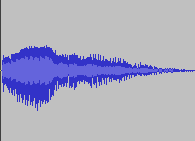
\includegraphics[width=.9\textwidth]{figs/original.png}
  \caption{Input example}
  \label{fig:inEx}
\end{subfigure}%
\begin{subfigure}{.32\linewidth}
  \centering
  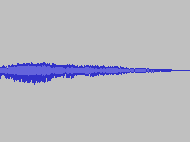
\includegraphics[width=.9\textwidth]{figs/lpf800.png}
  \caption{Output example}
  \label{fig:outEx}
\end{subfigure}
\begin{subfigure}{.32\linewidth}
  \centering
  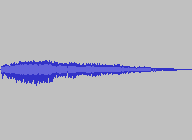
\includegraphics[width=.9\textwidth]{figs/lpf950.png}
  \caption{Generated}
  \label{fig:synthEx}
\end{subfigure}
\caption{The waveforms (a) and (b) are provided as examples, and DSP-PBE synthesizes a filter that produces (c).}
\label{fig:test}
\end{figure}

More creative applications?


\section{Background}

To give context for DSP-PBE, we first explain the traditional concept of programming by example~\cite{cypher93,lieberman01,synasc12}.
Programming by example (PBE) is a synthesis technique that automatically generates programs that coincide with given examples. An example is specified as a tuple of input and output values. Given a set $S= \{(i_1, o_1),\ldots, (i_n, o_n)\}$ of input/output examples, the goal is to automatically derive a program $P$ such that for every $j$, $P(i_j) = o_j$. 
Instead of writing code, the user provides a list of relevant examples and the synthesis tool automatically generates a program. In this way, the examples can be seen as an easily readable and understandable specification. However, even if the synthesized program satisfies all the provided examples, it still might not correspond to the user's intentions. Examples are, by nature, an incomplete specification.

PBE is a promising research direction that enables easy manipulation of data even for non-programmers~\cite{GulwaniHS12}. Recent work in this area has focused on manipulating fundamental data types such as strings~\cite{vldb12,icml13}, lists~\cite{FeserCD15,poseraZ15} and numbers~\cite{cav12}. The success and impact of this line of work can be estimated from the fact that some of this technology~\cite{flashFillPOPL} ships as part of the popular Flash Fill feature in Excel 2013~\cite{flashfill}.


The core difference between traditional PBE and DSP-PBE is in the application domain of Digital Signal Processing.
Digital Signal Processing (DSP) programming languages provide users with an interface to build signal processing programs in domain specific languages.
Some of these languages provide their own implementations of signal processing primatives, such as SuperCollider~\cite{supercollider}, CSound~\cite{csound}, and PureData~\cite{puredata}.
Other DSP languages provide alternative front-ends to these languages, such as Vivid~\cite{vivid}, which provides Haskell bindings to Supercollider.

Although many DSP languages are full featured enough to write general purpose programs, in this work we focus on the construction of DSP filters.
A DSP filter is, broadly speaking, any program that transforms a digital signal from one form to another.
An example of a DSP filter is a low-pass filter, which takes an input signal and generates an output signal that keeps frequencies below some frequency threshold, but removes frequencies above that threshold.

The most closely related work in audio signal processing is a technique called resynthesis~\cite{masri1996improved}.
Resynthesis is the process of decomposing a sound into its spectrogram, and then building a synthesizer to recreate a similar sound.
The limitation here is that resynthesis builds a generative synthesizer, which does not take into account any information about the components used to create the original sound.
This limitation means that resynthesis cannot be applied in a new context, whereas DSP-PBE allows us to construct a DSP program that can be used with various new input samples to create novel sounds. 
For example, DSP-PBE could be given a sample of a trumpet and a trombone, and the generated DSP program could be applied to a violin to hear what a violin sounds like if it was a trumpet that had been turned into a trombone.


\begin{figure*}[!ht]
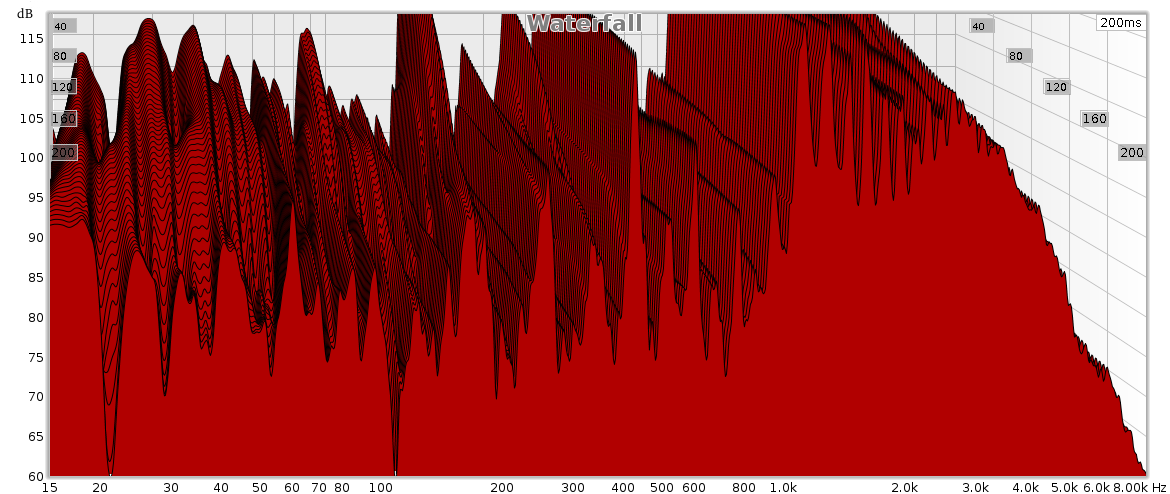
\includegraphics[width=\textwidth]{figs/waterfall} 
\caption{A waterfall plot of the \texttt{cartoon-spring.wav} from 0-200 ms between frequencies of 20-8000 Hz, where the height indicates the amplitude of each frequency. This plot was created with the REW tool~\cite{REWTool}.}
\label{fig:waterfall}
\end{figure*}

\section{Aural Distance}
\label{sec:distance}

As a distance metric, we used as a starting point the literature on acoustic fingerprinting~\cite{fingerprinting}.
Acoustic fingerprinting is the concept of creating a condensed, distinct summary of an audio file that can be used later to identify that audio file or to look it up in a database.
Acoustic fingerprints represent how the file will sound to the human ear regardless of how it is represented in a digital format.
There are numerous ways to develop acoustic fingerprints and companies like Shazam and Sound-Hound have developed complex algorithms to create accurate fingerprints even from low quality files recorded on a cellphone mic.
For this work, we used the work of Shazam~\cite{wang2003industrial} as an inspiration for our checker. \ruzica{where is this checker coming from?}


As an intuition, the psycho-acoustic identity of a sound file (how humans distinguish between one sound and the next) can be captured by taking every ``moment'' of audio, and listing the predominate frequencies for that slice of time.
This intuition can be represented with a waterfall plot, as shown in Figure~\ref{fig:waterfall}, which plots how the frequencies change over time.
A waterfall plot uses the Fast Fourier Transform (FFT) to convert an audio file into a list of spectrograms plotted over time.
In the Shazam method, the peaks are selected from each time slice of audio and used to create a ``constellation'' of peaks over time. 
This constellation is then used to build a hash that acts as a fingerprint to uniquely identify the audio sample.
We use a similar strategy by first performing a real Fast Fourier Transform on the audio file and then picking out the frequency peaks in each time frame.
However, the key difference in DSP-PBE is that we do not use the constellation as a hash for lookup in a database (as Shazam and SoundHound do), but instead, we need a distance metric between two constellations to provide a measure of how close we are to synthesizing the correct DSP filter.
Distance metrics are common in music synthesis tasks, for example, in the generation of jazz improvisations, where the improvisation should stay close by some measure to the original melody~\cite{donze2014machine}.

Fast Fourier Transforms (FFT) are the key to a good acoustic fingerprint.
The FFT, however, cannot be taken as a blackbox in our application.
The two factors we need to consider are 1) the window-size for how many samples will be used to calculate the FFT, and 2) the bin size which roughly speaking, defines the resolution of the FFT.

Each return element is a frequency \textit{bin}, and depending on the scale of your return array the size of these bins varies.
In order for each bin to correspond to 1 Hz the size of the return vector must be equal to the sampling frequency (44,100 Hz).
If each bin is not 1 Hz, the effects of spectral leakage will be seen.
This occurs when the bins do not correspond to the exact frequency peaks of the sound.
The amplitude from the peaks that fall in between bins will \textit{leak} over into the closest bin and create a distorted spectrogram.
For this reason we had to adjust the size of the FFT return arrays to be 44,100.
Although this slows down the process of FFT, it provides the most accurate representation of the sound and for our purposes frequency accuracy is paramount.

With our constellations created from the waterfall plot, we constructed a \texttt{dist} function in measuring the aural distance and is faithful to the psycho-acoustics of the human ear.
Our implementation takes the Euclidean distance of the peaks in a time slice on the frequency-amplitude axis.
In order to define this distance more formally, we introduce the notation $c@t$ to indicate selecting time slice $t$ from constellation $c$.
We also use the function $peak:: Int \to Constellation \to Peak$ to select a peak from a constellation, where the peaks are in sorted order based on frequency.
Then, for an audio clip $x$ and an audio clip $y$, and a function $toC :: Audio \to Constellation$ to transform the audio clip into a constellation with $ts$ time slices and $p$ peaks in each time slice:

\begin{align*}
\sum_{t=0}^{ts}\ \sum_{i=0}^{p} euclid\Big(\ &peak(i,toC(x)@t), \\ &peak(i,toC(y)@t)\ \Big)
\end{align*}

Note that this definition requires the audio clips to be temporally aligned, which is not always a fair assumption in the real world. We leave the exploration of a temporal offset between two example audio samples to future work.

As a sanity check that this distance metric matches the psycho-acoustic definition of distance, we used the test cases listed in Table~\ref{table:dist}.

\begin{table*}[!h]
\centering
\begin{tabular}{|l | c | c|} 
 \hline
 Test Name \& Expected Result & Value 1 & Value 2 \\
 \hline
 \hline
 Identity & \multirow{2}{*}{(PianoC, PianoC) = 0} & \multirow{2}{*}{NA}\\ 
   \quad Value 1 = 0 &  & \\
 \hline
 Associativity & \multirow{2}{*}{(PianoC, PianoCSharp) = 5.635} & \multirow{2}{*}{(PianoCSharp, PianoC) = 5.635} \\
   \quad Value 1 = Value 2  & & \\
 \hline
 Associativity & \multirow{2}{*}{(PianoC, HornCSharp) = 20.500} & \multirow{2}{*}{(HornCSharp, PianoC) = 20.500} \\
   \quad  Value 1 = Value 2 & & \\
 \hline
 Filter less than pitch & \multirow{2}{*}{(PianoC, PianoFilterC) = 3.749} & \multirow{2}{*}{(PianoC, PianoCSharp) 5.635} \\ 
   \quad Value 1 $<$ Value 2 & & \\
 \hline
 Filter less than pitch+instrument & \multirow{2}{*}{(PianoC, PianoFilterC) = 3.749} & \multirow{2}{*}{(PianoC, HornCSharp) 20.500} \\
   \quad Value 1 $<$ Value 2 & & \\
 \hline
 Pitch less than pitch+instrument & \multirow{2}{*}{(PianoC, PianoCSharp) = 5.635} & \multirow{2}{*}{(PianoC, HornCSharp) 20.500} \\
   \quad Value 1 $>$ Value 2 & & \\
 \hline
\end{tabular}
\caption{Test cases to evaluate distance metric. The exact values are only important in relationship to the others.}
\label{table:dist}
\end{table*}


The goal in the synthesis procedure is to find a DSP filter program, $F$, such that \texttt{dist$(O, F(I))$ = 0}.
However, in practice the DSP-PBE Synthesizer can only get us so close to this metric and we instead just minimize this distance.
To do this, the user specifies a default threshold distance for the aural distance.
The threshold distance defines how close is acceptably close, and can be changed by the user depending on their needs or requirements.


\section{Search}
\label{sec:search}

Search techniques for programming by example have been the subject of intense research~\cite{?,?,?}.
As the search space of possible program is extremely large, search procedures must be exceptionally efficient. 
As a first foray into DSP-PBE, we restrict ourselves to only synthesizing low-pass and high-pass filters.
These two filters have the key property that they are quasi-commutative - when the thresholds of these filters do not overlap, applying a low-pass and then a high-pass is the same as applying a high-pass and then a low-pass.
We leave the exploration of non-commutative filters (for example, delay lines or ring filters) to future work.

\subsection{Gradient Descent}

One trouble with this approach is that we have lots of local minimums in the space of optimization.
Take the example of trying to learn a low-pass filter threshold.
If our initial threshold is too low (cutting off too much), and just on the other side of the threshold is a frequency we need, SGD will easily send us in that direction.
However, if the spectrogram of waveform has a frequency spectrum that is mostly inactive, SGD will detect a plateau and tell us we have found a global minimum, when in fact we are stuck in a local minimum.
We may be able to use some randomized restarting to hop over these.

\subsection{Refinement Type Driven Synthesis}

In order to find an initial value for gradient descent, we can use refinement types.
The use of formal methods in music has been explored previously~i
Refinement types are a way of giving an abstract description of the behavior of a function. 
For example, we given the function 
%
\texttt{map::[a]} $\to$ \texttt{[b]}
%
we can further provide a refinement types that captures some properties of the behavior of this function:

\texttt{f::xs:[a]} $\,\to\,$ \texttt{ys:[b]} \textbar \texttt{ length xs == length ys}

\noindent In this case, the refinement type describes that the length of the lists are still equal after applying the \texttt{map} function.

In a similar style for DSP, we can write predicates about the filters available to us during synthesis. 
For example, a low-pass filter could be described as the refinement type that says the amplitude of the frequencies greater than the threshold frequency have decreased in the output Audio.

\texttt{lpf::t:Float} $\,\to\,$  \texttt{xs:Audio} $\,\to\,$ \texttt{ys:Audio} \textbar
\texttt{ ($\forall$$f_1$ $\in$ spectrogram(xs)}, \texttt{ $\forall$$f_2$ $\in$ spectrogram(ys))}:  \centerline{\texttt{(}$f_1$ $\textgreater$ \texttt{t}  $\land$  $f_2$ $\textgreater$ \texttt{t}  $\land$  $f_1$ == $f_2$ $\implies$ \texttt{(amp($f_1$) $\textgreater$ amp($f_2$))}} ~\\
Where \texttt{t} represents the level at which the lowpass filter is applied, \texttt{spectrogram} represents the spectrogram of the sound sample, $f_i$ represents a frequency, and \texttt{amp()} represents the amplitude of the frequency. This refinement type can be abbreviated into \texttt{$r_{lpf}$(t, xs, ys)}, a predicate on a threshold frequency \texttt{t} and the two audio files \texttt{xs, ys}. \\ \\
Additionally, a high-pass filter could be described as the refinement type that says the amplitude of the frequencies less than the threshold frequency have decreased in the output Audio. \\

\centerline{ \texttt{hpf::t:Float} $\,\to\,$  \texttt{xs:Audio} $\,\to\,$ \texttt{ys:Audio} \textbar }
\centerline{\texttt{ ($\forall$$f_1$ $\in$ spectrogram(xs)}, \texttt{ $\forall$$f_2$ $\in$ spectrogram(ys))}: } \centerline{($f_1$ $\textless$ \texttt{t}  $\land$  $f_2$ $\textless$ \texttt{t}  $\land$  $f_1$ == $f_2$ $\implies$ \texttt{(amp($f_1$) $\textgreater$ amp($f_2$))}} ~\\
Where \texttt{t} represents the level at which the highpass filter is applied, \texttt{spectrogram} represents the spectrogram of the sound sample, $f_i$ represents a frequency, and \texttt{amp()} represents the amplitude of the frequency. This refinement type can be abbreviated into \texttt{$r_{hpf}$(t, xs, ys)}, a predicate on a threshold frequency \texttt{t} and the two audio files \texttt{xs, ys}.

\subsection{Combination of Search Algorithms}

One hypothesis as to how we would combine both algorithms would be through a feedback loop. We will use the refinement types to select a filter with a parameter. We then send that information into gradient descent to find a more precise filter representation (more accurate parameter measure). We will then apply this filter with the new parameter value from gradient descent to the input sound sample. Next, we will send this new sound sample $(F(I))$ and the original output sound sample $(O)$ to the aural distance function \texttt{dist}. If the \texttt{dist} function returns a value lower than the threshold distance given by us or the user, then we will accept that filter and return it to the user. If it is not, we will attempt to refine our parameter for the filter. An example of this can be seen in the diagram below: 

%\begin{figure}[!htb]
%\centerline{\includegraphics[width=\textwidth]{CPSC2}}
%\caption{Flow diagram of the DSP-PBE Synthesizer}\label{fig:image6}
%\end{figure}\\ 

This loop could become more complicated as multiple filters could be applied to one sound sample once the parameter has been tuned to the best value. This idea will be discussed later in this paper.

\subsubsection{Filter List}

For the DSP-PBE problem on sound samples, we will have a list of filters and corresponding refinement types. The goal for the filter list is to have enough variance in the filters in the list so that gradient descent can then refine the parameter for the filter (finding the global minimum and not getting caught at a local minimum), and no one value of the filter parameter will be overlooked. However, we are going to have to strike a balance between accuracy and length of filter list because the longer the filter list is, the longer it will take to search through all of the filters and corresponding refinement types. As an example, a filter list with only low pass filters would look as below:

\begin{enumerate}
{\setlength\itemindent{150pt} \item{\texttt{lpf($\delta$, xs, ys)}}}
{\setlength\itemindent{150pt} \item{\texttt{lpf(2$\delta$, xs, ys)}}}
\end{enumerate}
\centerline{\bm{$\vdots$}} ~\\
Where $\delta$ is the smallest variance necessary for gradient descent to find the global minimum from this delta and not a local minimum, and the largest variance necessary so any two filters would not overlap. This delta will need to be discovered by practice. 

\subsubsection{Ordering of Refinement Types}

As stated above, the longer the filter list becomes, the longer it will take to search through the list to find a refinement type that holds with the spectrogram of the input and output sound samples. In order to combat this, we could order the filters accordingly, to decrease the time it takes to search through them. We could also attempt to increase the accuracy of the parameters for the filters we know hold on our sound samples. \\ \\
Let's take our filter list created above. For some $\delta$ not yet discovered, a filter list with only lowpass filters will look as follows:

\begin{enumerate}
{ \item{\texttt{lpf($\delta$, xs, ys)}}}
{ \item{\texttt{lpf(2$\delta$, xs, ys)}}}
\end{enumerate}
\centerline{\bm{$\vdots$}} 
\begin{enumerate}
{ \item{\texttt{lpf(maxf - 2$\delta$, xs, ys)}}}
{ \item{\texttt{lpf(maxf - $\delta$, xs, ys)}}}
\end{enumerate}
As stated above, we know a low-pass filter could be described by a refinement type stating that the amplitude of the frequencies greater than the threshold frequency value have decreased in the output Audio. For this reason, we know that if any lowpass filter is applied in our output sound sample, the refinement type with the greatest threshold frequency in our filter list will hold for our input and output spectrograms (in this case \texttt{lpf(maxf - $\delta$, xs, ys)}). Formally, we know: \\ \\
\centerline{\texttt{xs::Audio $\land$ ys::Audio $\land$ $r_{lpf}$(t, xs, ys) $\implies$}} \\
\centerline{\texttt{ $\forall$ t' $\textgreater$ t. $r_{lpf}$(t', xs, ys)}} ~\\
So, to attempt to decrease the number of filters tried, we could test the greatest threshold frequency lowpass filter in the filter list, and if it does not hold, we can skip all other lowpass filters in the list. The opposite would hold true for highpass filters: \\ \\
\centerline{\texttt{xs::Audio $\land$ ys::Audio $\land$ $r_{hpf}$(t, xs, ys) $\implies$}}\\
\centerline{\texttt{ $\forall$ t' $\textless$ t. $r_{hpf}$(t', xs, ys)}} ~\\
As we create more refinement types for other filters, we can create different orders to decrease the number of refinement types needed to test to find one that hold for our input and output spectrograms. \\ \\
If we want to increase the accuracy for our refinement types, the order for the filter list will need to be different. If we look at the example filter list above, we would want to start from the lowest threshold frequency filter in the list (\texttt{lpf($\delta$, xs, ys)}) and increase the threshold frequency level from there. This way, we won't skip over our threshold frequency at any point (and therefore end up with a local minimum in gradient descent rather than the global minimum). For highpass filters, we would again want to do the opposite of the lowpass filters and start with the highest threshold frequency value available and decrease that value when searching for the optimal threshold frequency level. Again, we would hopefully be able to make these optimizations with other filter/refinement type additions. This will be the easiest way to increase accuracy or decrease time (or a combination of both) to optimize our DSP-PBE tool.

\subsubsection{Application of Refinement Types}

Given our ordered filter list, we can update our flow chart from Figure~\ref{fig:image6}. The choice of a filter will depend on the order described in the previous section. First, we check the worst case scenario for each filter type. If the worst case scenario for one filter holds, then we go back and test the filters in the order that will correctly increase accuracy for that filter. Otherwise, we skip that filter type all together and move on to the next one. The flow chart below describes the choice of a refinement type from the filter list:
%\begin{figure}[!htb]
%\centerline{\includegraphics[scale = 0.55]{CPSC490FlowFLChoose}}
%\caption{Flow diagram of refinement type choice}\label{fig:image7}
%\end{figure}\\ 

Only after finding the correct refinement type parameter will we send that filter corresponding to it to gradient descent to further optimize the parameter. Finally, we check the aural distance of the filter on the input sound sample ($F(I)$) and the output sound sample ($O$), and complete the feedback loop according to the results. The updated flow chart is below:

%\begin{figure}[!htb]
%\centerline{\includegraphics[width=\textwidth]{CPSC}}
%\caption{Flow diagram of DSP-PBE Synthesizer with filter list}\label{fig:image8}
%\end{figure}

\begin{comment}
Once an order has been found that best optimizes the refinement type list, we then need to apply the refinement types. In order to apply the refinement type, we will go through our refinement type list and test each if each one holds true on the spectrogram of the input and output sound samples, skipping the ones accordingly as described above. We will start with the refinement types of the same type and check different parameter levels after that. Once we know a refinement type doesn't work, we can remove it from the list of refinement types. This will decrease the time it takes to look up refinement types if we need to apply more than one filter to our sound sample. Once we find a refinement type that works, we apply the filter corresponding to that refinement type to the input sound file and send that file to gradient descent. We will then come up with a threshold for the lowpass and highpass filter and send that threshold and filter to the aural distance function.
\end{comment}

\subsubsection{Combination of Refinement Types}

When applying refinement types and the filters corresponding to them, just one may not be enough. In this paper, we are keeping things simple with just lowpass and highpass filters. However, in theory, we could have a multitude of filters being applied over each other (ex. lowpass, delay, white noise, etc.). So, in order for DSP-PBE to work in practice, we need to be able to apply more than one filter to our sound sample and therefore, more than one refinement type to the spectrogram of that sound sample. \\ \\
We can first find any one filter that fits our parameters. For example, let's say a refinement type of a lowpass filter holds true. As described above, we will optimize this filter to have a threshold frequency closest to the actual threshold frequency of the output filter and send this filter and threshold frequency  to gradient descent. Gradient descent will hopefully find the global minimum and return a threshold frequency and filter to us ($F$). However, even though this optimized filter returned an answer, the aural distance between $F(I)$ and $O$ could still be greater than the aural distance threshold. So, next, we would need to try and decrease the aural distance between these two filters. One way we can do this is by adding another filter on top of $F(I)$. \\ \\
In order to do this, we must apply the filter that corresponds to the first refinement type used ($r_1$) to the input sound sample, creating a new sound sample, $s_{new}$ (where $s_{new}$ = $F(I)$). We must then return to our filter list and test different filters on $s_{new}$ as the input. The goal would be to see if any filter holds for $s_{new}$ as the input sound sample and the original output sound sample as the output. Basically, our new goal would be to find a new filter ($F_2$) such that \texttt{dist}$(F_2$$(F(I)), O)$\texttt{ = 0} or \texttt{dist}$(F_2$$(s_{new}), O)$\texttt{ = 0}. If a second filter is found (and coincidentally a second refinement type, $r_2$), then we will send the two filters used in conjunction to gradient descent, and then after, to the distance function, to see if they can return an aural distance below the threshold distance given by the user. \\ \\
The refinement type for a combination of filters and therefore a combination of refinement types would look as follows: \\

\centerline{$r_{combined}$:: \texttt{x:Audio} $\,\to\,$ \texttt{y:Audio} \textbar \texttt{ $\exists$z. $r_1$(x, z) $\land$ $r_2$(z, y)}} ~\\
where \texttt{z} is $s_{new}$, \texttt{x} is the original input sound sample, \texttt{y} is the output sound sample, $r_1$ is the first refinement type, and $r_2$ is the second refinement type. \\ \\
This process can be repeated as many times as necessary as many filters could be applied to an input sound sample to obtain the output sound sample. 
\begin{comment}
The new feedback loop would look something like this: \\
\includegraphics[width=\textwidth]{CPSC490Flow2.png}
\end{comment}






\section{Evaluation}

To evaluate our approach, we apply our synthesis algorithm to two sets of input/output examples.
The first set captures the use case of \ourTool where a user wants to model real world sounds.
This set consists of trumpet sounds with various mutes.
The second set of example input/output we run \ourTool on focuses on more creative applications.
Here we attempt to transform whitenoise into various clips from Brian Eno's Music for Airports.

The results of running \ourTool on the trumpet mute sounds benchmarks are reported in Table~\ref{table:eval}.

We need to normalize all files as the distance metric is amplitude analysis.

\begin{table}
\begin{tabular}{|l|l|c|c|c|}
\hline
\textbf{Input} & \textbf{Filter} & \textbf{dist(o, $f$(i))} & \textbf{Time (sec)}
\csvreader{results/farm.csv}{}
{\\ \hline \csvcoli & \csvcolii & \csvcoliv & \csvcolvi}
\\ \hline
\end{tabular}
\caption{Demonstrating the accuracy of the user provided refinements for the initial filter.}
\label{table:evalInit}
\end{table}

\begin{table*}[]
\begin{tabular}{|l|l|c|c|c|}
\hline
\textbf{Input} & \textbf{Output} & \textbf{dist(o, $f$(i))} & \textbf{Structural Attempts} & \textbf{Time (sec)}
\csvreader{results/trumpet.csv}{}
{\\ \hline \csvcoli & \csvcolii & \csvcoliv & \csvcolv & \csvcolvi}
\\ \hline
\end{tabular}
\caption{Evaluation on a set of benchmarks.}
\label{table:eval}
\end{table*}




\section{Refinement Type Driven Synthesis}
\label{sec:rtypes}

In order to find an initial value for gradient descent, we could use refinement types.
In this section we explore a possible optimization for selecting an initial DSP program for gradient descent.
This has not yet been implemented, but we present the theory behind the approach.

\subsection{Refinement Types for DSP}
\label{sec:retypeSearch}
Refinement types are a way of giving an abstract description of the behavior of a function. 
For example, given the function 
%
\texttt{map :: [a]} $\to$ \texttt{[b]}
%
we can further provide a refinement types that captures some properties of the behavior of this function over values:
%
\begin{align*}
\texttt{f :: xs:[a]} \to\ \texttt{ys:[b]}\ \mid \texttt{ length xs == length ys}
\end{align*}

\noindent In this case, the refinement type describes that the length of the lists are still equal after applying the \texttt{map} function.

In a similar style for DSP, we can write predicates about the filters available to us during synthesis. 
For example, a low-pass filter could be described as the refinement type that says the amplitude of the frequencies greater than the threshold frequency have decreased in the output Audio.
For brevity in notation, we will only treat a single time slice from the waterfall plot here, but the concept generalizes when quantified over all time slices as well.
%
\begin{align*}
  &\texttt{lpf :: t:Float} \to  \texttt{xs:Audio} \to\ \texttt{ys:Audio}\ \mid \\
  &\forall f_1 \in  \texttt{spectrogram(xs)}.\ \forall f_2 \in \texttt{spectrogram(ys)}. \\
  &(f_1 > \texttt{t}  \land  f_2 > \texttt{t}  \land f_1 == f_2) \implies \texttt{amp}(f_1) > \texttt{amp}(f_2)
\end{align*}

Where \texttt{t} represents the level at which the lowpass filter is applied, \texttt{spectrogram} represents the spectrogram of the sound sample, $f_i$ represents a frequency, and \texttt{amp()} represents the amplitude of the frequency. 

Additionally, a high-pass filter could be described as the refinement type that says the amplitude of the frequencies less than the threshold frequency have decreased in the output Audio.
%
\begin{align*}
  &\texttt{hpf :: t:Float} \to\ \texttt{xs:Audio} \to\ \texttt{ys:Audio}\ \mid \\
  &(\forall f_1 \in \texttt{spectrogram(xs)}. \forall f_2 \in \texttt{spectrogram(ys)}). \\
  &(f_1 < \texttt{t} \land f_2 < \texttt{t} \land f_1 == f_2) \implies \texttt{amp(}f_1\texttt{)} > \texttt{amp(} f_2 \texttt{)} 
\end{align*}

Notice that in these refinement types, we only need to calculate the spectrogram for the input and output statically.
As opposed to the current technique of generating filters, applying them, and the calculating the aural distance, this approach is relatively static.
We could quickly check many threshold values over the input and output examples.
This will only yield a rough boolean estimation of whether this threshold should even be considered, but this is enough information for us to select an initial program to pass to our gradient descent algorithm.
As the search for an initial filter takes roughly 40 seconds out of our current benchmarks, this could dramatical increase the speed of synthesis.

\subsection{Combination of Search Algorithms}

Beyond just using the refinement types to select an initial program for gradient descent, we can use refinement types in as part of the main search strategy as well.
We briefly describe here a way to use refinement types in combination with gradient descent to handle more complex combinations of DSP filters.
So far in our work (\textit{c.f.} Sec.~\ref{sec:eval}) we have synthesized filters with a fixed form - all our solutions use a single low-pass filter, and a single high-pass filter.
Ideally, we would be able to synthesize solutions that use any arbitrary combination of filters.
In order to do this, we would need an iterative solution that can find one filter at a time.

In this approach, given input example \texttt{x:Audio} and output example \texttt{y:Audio}, we would first find a filter \synthFilter' using the approach described in Sec.~\ref{sec:search} and Sec.~\ref{sec:rtypeSearch}.
We will say that this \synthFilter' has the refinement type $r_1$.
However, this filter might not return a satisfactory result.
We could then continue the search using the output of \synthFilter'\texttt{(x)} as the new input example, \texttt{z:Audio}.
Now the synthesis task is to find a filter \synthFilter'' (with refinement type $r_2$) using input example \texttt{z:Audio} and output example \texttt{y:Audio}.
Essentially, \synthFilter' has gotten us the first half of the way, and \synthFilter'' will get us the second half of the way.
With this, we can start to use more information rich refinement types, such as below:
%
\begin{align*}
\synthFilter \texttt{:: } & \texttt{x:Audio} \to\ \texttt{y:Audio}\ \mid \\
   & \exists \ \texttt{z:Audio}.\ r_1\texttt{(x,z)} \land r_2\texttt{(z,y)}
\end{align*}


\section{Future Work and Conclusions}

The main contribution of this paper is to pose the problem of DSP-PBE.
While we have presented a prototype implementation of a DSP-PBE tool, this primarily functions as a proof-of-concept.
There remains significant room for optimization in both the distance calculation and the search algorithm.

Although with the current tool, synthesis times presented might be prohibitively slow for many use cases, we should be encouraged by progress in other domains of program synthesis.
In the SyGuS program synthesis competition, which has run for 4 years, tools have seen an exponential speed up and increase in the range of programs that can be synthesized.
As one example, in the 2014 competition the \texttt{LinExpr\_eq1.sl} benchmark was only solved by one tool, and took 1128 seconds in 2014~\cite{sygus2014}.
In the 2017 competition, the same benchmark was solved by all tools, with the fastest taking only 199 seconds~\cite{sygus2017}.




\bibliography{nime-references}  

%%% Place this command where you want to balance the columns on the last page. 
%\balancecolumns 

% That's all folks!
\end{document}
